\chapter{Test af equalizer}\label{sec:test_eq}




\emph{I dette kapitel bliver der redegjort for testforløbet af equalizeren. Der bliver brugt en Bode 100 til måling af equalizerens overførselsfunktion. På denne måde kan det bevises om equalizerens profiler fungerer korrekt.}

\section{Equalizer filtre}


Liste over presets hvis amplitude spektrum måles.

Måling af Amplitude og fase med bode100 for følgende presets:
\begin{enumerate}[noitemsep,nolistsep]
    \item Equalizeren slået fra.
    \item Megafon preset.
    \item Bass boost preset.
    \item High boost preset.
    \item Rock preset. 
    \item 1k notch preset. \\
\end{enumerate}

Måling med funktions generator. Scoop på indgang, udgang.
EQ med 1k notch presetet. 
Send 1k sin bølge ind. 


\subsection{Målinger}


\begin{figure}[h]
\centering
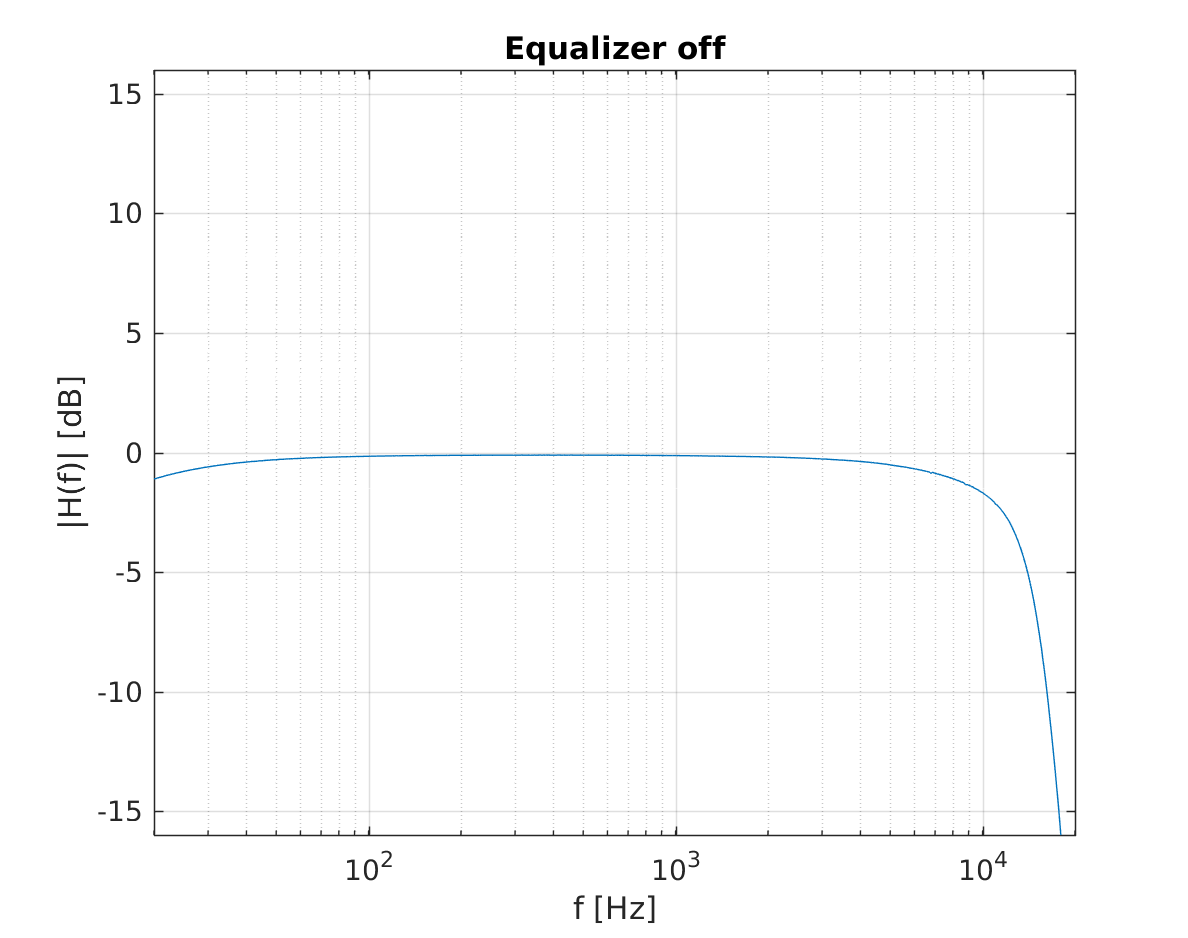
\includegraphics[]{matlabdemo/test/eq_off.png}  
\caption{Måling af hele systemet uden equalizer slået til.}
\end{figure}


\begin{figure}[h]
\centering
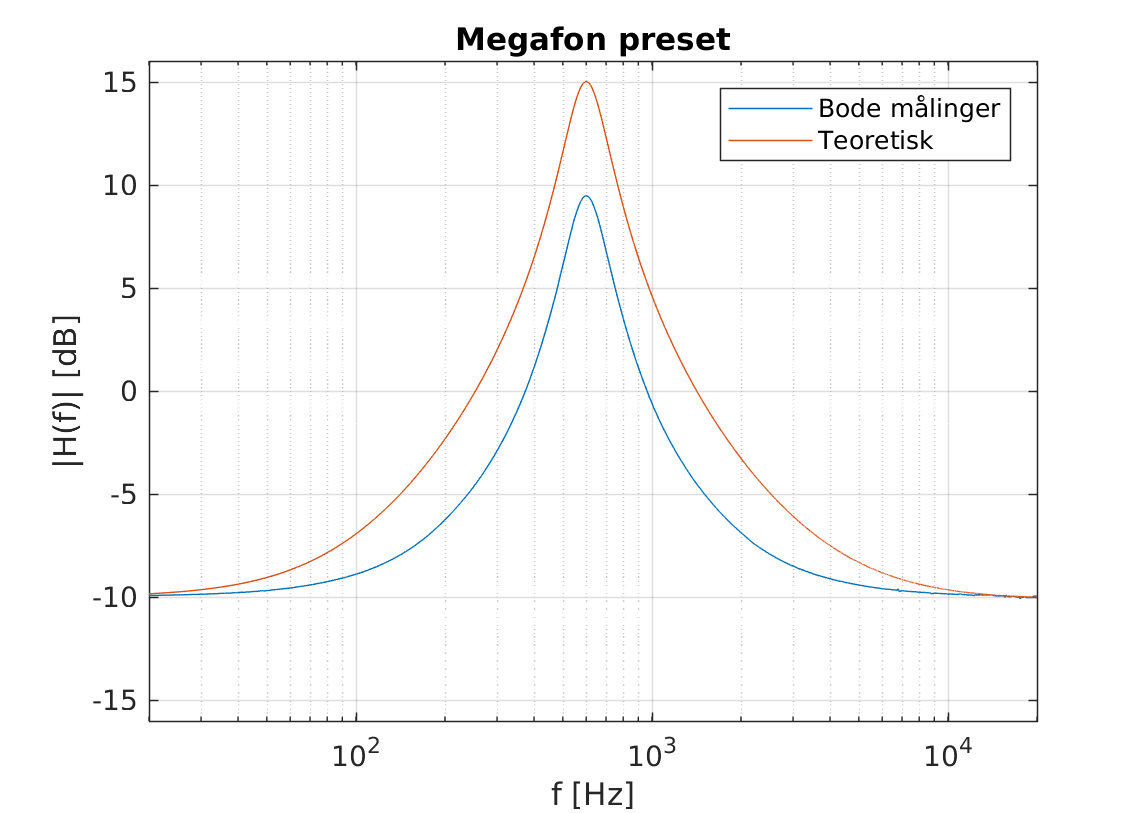
\includegraphics[]{matlabdemo/test/eq_megafon.png}
\caption{Måling af megafon preset.}
\end{figure}

\begin{figure}[h]
    \centering
    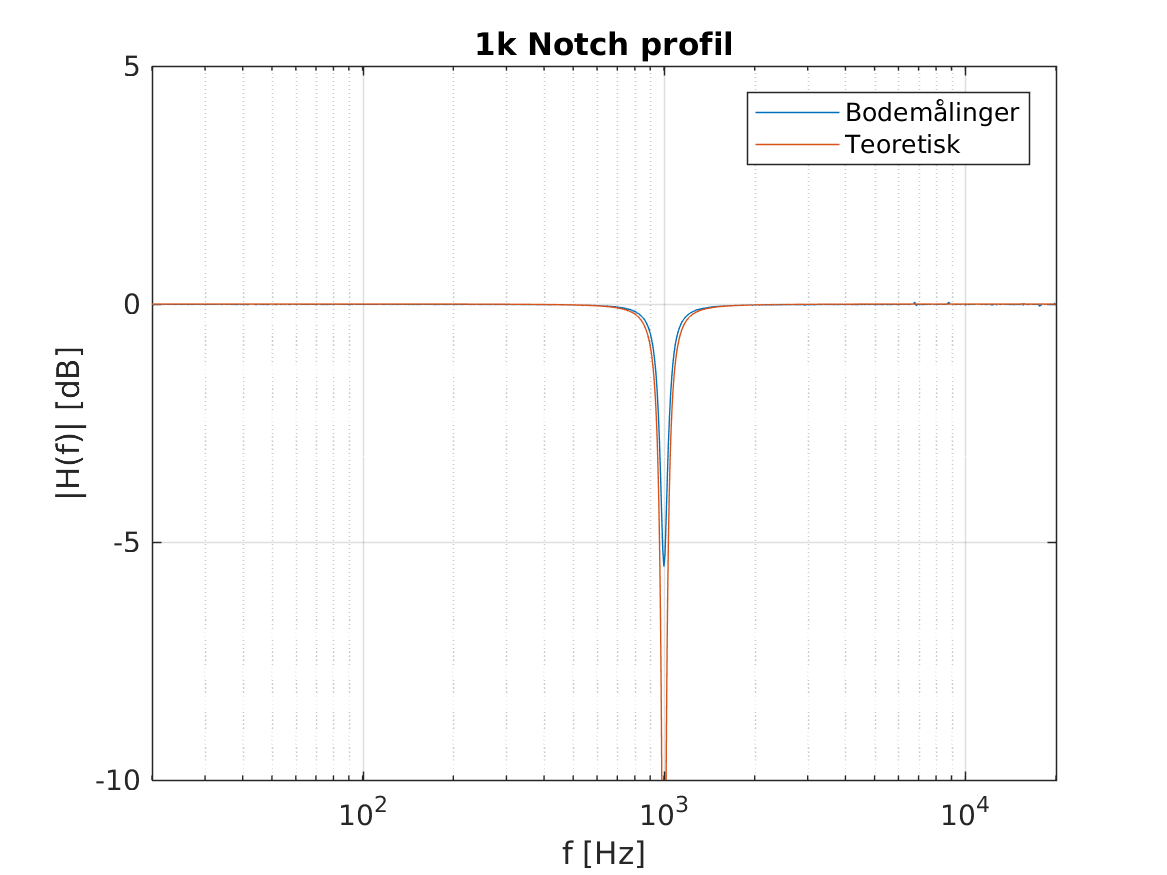
\includegraphics[]{matlabdemo/test/eq_1knotch.png}
\end{figure}

\begin{figure}[h]
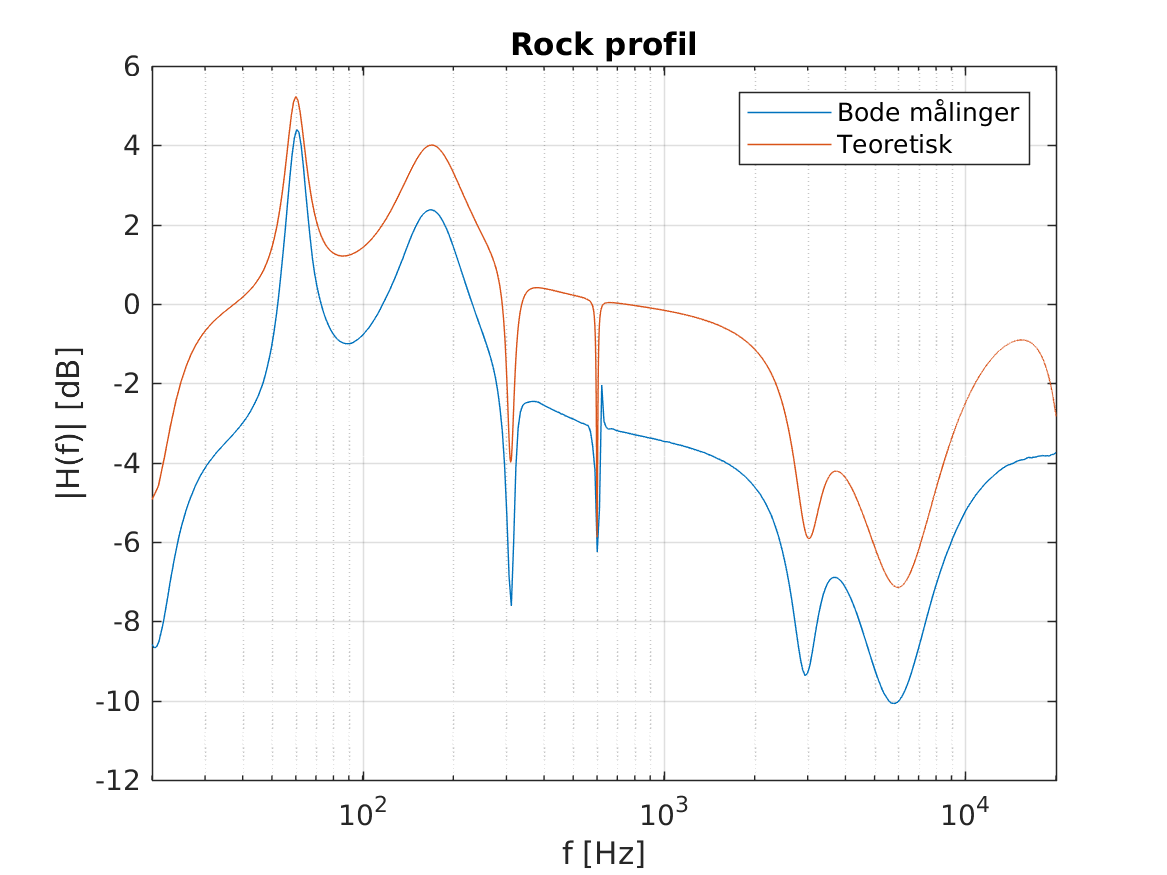
\includegraphics[]{matlabdemo/test/eq_rock.png}
\caption{Sammenligning mellem den teoretiske rock profil og den målte.}
\end{figure}



Derudover skulle "1k notch" preset'et måles med et oscilloskop på indgangen og udgangen, mens en funktionsgenerator sendte en $1$\kilo\hertz bølge ind på indgangen. Dette skulle eftervise om preset'et gjorde præcist hvad det skulle. \\

\section{Udførelse}
For at måle overføringsfunktionen sættes Bode 100'ens output til indgangen på equalizeren. CH1 sættes også til indgangen. CH2 sættes til udgangen og målingen foretages for samtlige af ovenstående presets. 

\begin{figure}[h!]
	\centering
	\includegraphics[width=15cm]{billeder/setup}
	\caption{Målingssetup med Bode 100}

\section{Resultater}
Som det ses på figur \ref{fig:rock_test} ligger testresultaterne meget tæt på de teoretiske. Det vurderes at dette ligger inden for fejlmargin. Målingerne blev foretaget med et indgangssignal på 4dBm, for at sikre at ingen af profilerne overstyrede.

\begin{figure}[h!]
	\centering
	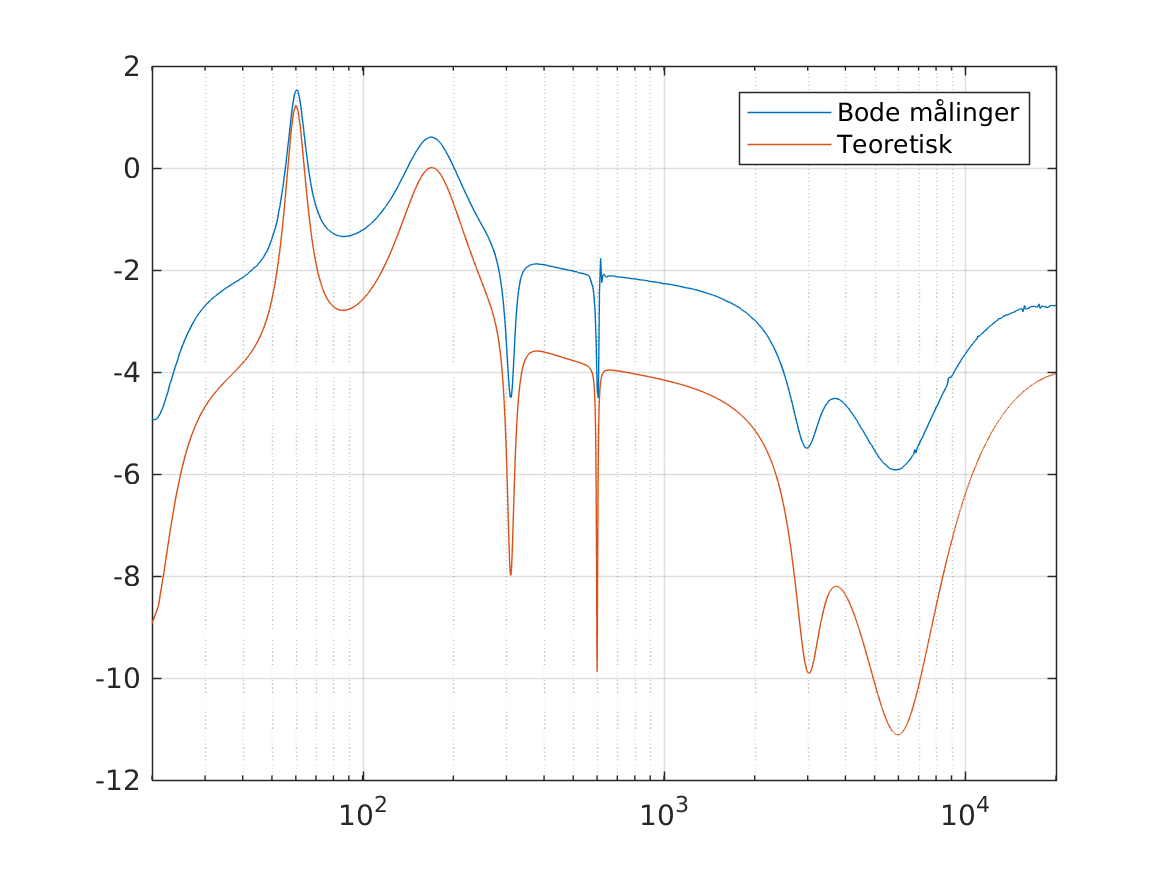
\includegraphics[width=15cm]{billeder/rock_test}
	\caption{Sammenligning af "Rock"-profilen, teoretisk (orange) og måling (blå)}
	\label{fig:rock_test}
\end{figure}

Der blev dog, vha. testene, fundet en fejl i DSP-beregningerne, som derfor kunne rettes. Der blev opdaget at den angivede frekvens i profilen altid var fordoblet på udgangen. Dette var på grund af at udregningen skulle ganges med $\frac{f_s}{2}$ i stedet for $f_s$.

\end{figure}

